
%(BEGIN_QUESTION)
% Copyright 2010, Tony R. Kuphaldt, released under the Creative Commons Attribution License (v 1.0)
% This means you may do almost anything with this work of mine, so long as you give me proper credit

Determine how you would connect a 4-20 mA loop calibrator to the following level alarm system in order to test the alarm unit (LAH-37) to see if the alarm activates at its trip point of 11.5 feet:

$$\includegraphics[width=15.5cm]{i03687x01.eps}$$

\begin{itemize}
\item{} Identify where you would connect the loop calibrator into the circuit (a simple sketch would be ideal, or you could describe all connections)
\item{} Identify the proper mode for the loop calibrator ({\it source}, {\it simulate}, or {\it measure})
\item{} Calculate the proper amount of loop current to make the alarm unit ``think'' the transmitter is measuring 11.5 feet of liquid level
\end{itemize}


\underbar{file i03687}
%(END_QUESTION)





%(BEGIN_ANSWER)

5 points for correct loop calibrator usage ({\bf transmitter disconnected, loop calibrator connected in parallel with cable, set to ``simulate'' mode}), 5 points for current value of {\bf 18.15 mA}.

%(END_ANSWER)





%(BEGIN_NOTES)

{\bf This question is intended for exams only and not worksheets!}.

%(END_NOTES)


